% !TeX root = SA_Rockstroh_Main.tex
\chapter{Vorbetrachtung} 
% Vorwissen:
% - Grund des Kataloges
% - Prinzipielle Funktion/Nutzen
%
% =-- Vor dem Schreiben angedachter Inhalt ---=
%Inhalt:\\
%Grundgedanken zu Modellkatalog. Ansprüche. Wünsche bzgl. Funktionsumfang und Anwendbarkeit, Prinzip: aufwändiges Hinzufügen, einfaches Anwenden \\
%Ist-Stand: Was gibt es für vergleichbare Kataloge/Projekte? + Bewertung dieser\\
%Beschreibung der aktuellen Situation zur Modellfindung --> Zeitintensive suche nach Publikationen, nur ausgewählte Eigenschaften benannt und untersucht, teils uneinheitliche, unübersichtliche, komplexe Modelldarstellung, Reproduzierbarkeit der Implementierung der Ergebnisse einer Publikation aber auch allein schon des Modells oft sehr schwierig \\
%Grundüberlegungen zu den nützlichen Elementen des Kataloges: \\ Modell als Art Datenbankeintrag (Erschließbarkeit über Suche --> Einheitliche Attributsnamen (--> KS) + Bedeutung, Erweiterbarkeit), \\ Textuelle (semantische?) Modelldarstellung mit einheitlicher Struktur und Modellnotation, \\einheitliche Implementierung die einfache Nutzbarkeit der Modelle erlaubt \\
%Umsetzung der einzelnen Elemente: \\
%Metadata-File: Struktur aus ACKRep übernommen - leicht Angepasst \\
%Klassifikationssystem: Semantische, ontologische Ausarbeitung des auf Modelle anwendbaren Teilbereich der Regelungstheorie, Anforderungen explizit? --> Graphentheorie, Finden einer fachlich korrekten, eindeutigen - in Bezug auf Ontologie selbst und auf Anwendung auf Modelle - und verständlichen Darstellung (Beispiel Polynom --> linear/nicht-linear) und Namensgebung (strictly\_non\_linear)\\ 
%Textuelle Repräsentation: Struktur abgeleitet aus (guten) Publikationen[Referenzen], sinnvolle Informationsreihenfolge, Offenhaltung von Gestaltungsspielraum in Anbetracht des Umfangs der Regelungstechnik \\ 
% =-- Vor dem Schreiben angedachter Inhalt ---=
%
%Alternative Struktur: 	Section: Aktueller Stand (der Modellsuche und von Modellkatalogen)
%						Section: Prozess der Katalogerstellung/ Grund-/Vorgedanken zum Katalog
%						Subsections: Anforderungen - Kurze Diskussion was sinnvoll, Struktur, Elemente

%TODO: Neue Formulierung für Einstieg in Ch:1
Der in \ref{Ch:Ergebnisse} vorgestellte Katalog und dem dazugehörigen Klassifikationssystem ist das Resultat vieler Entscheidungen. Dem ist eine Recherche von Literatur mit regelungstechnischen Modellen voraus gegangen. Das Kapitel beginnt mit einer Erklärung zu den Begriffen \textit{System} und \textit{Modell}. Anschließend wird in \ref{Ch:Vorbetrachtung:Sec:CurrentState} der aktuelle Stand der Modellrecherche und vorhandener Modellsammlungen vorgestellt. Danach werden in \ref{Ch:Vorbetrachtung:Sec:Anforderungen} die Anforderungen für den Katalog formuliert und getroffene Entscheidungen vorgestellt, die zur Erfüllung der Anforderungen beitragen sollen. Bevor in \ref{Ch:Vorbetrachtung:Sec:KS} die wichtigsten Entscheidungen zur Erstellung des Klassifikationssystems vorgestellt werden, gibt es in \ref{Ch:Vorbetrachtung:Sec:Wissensrepräsentaionen} noch eine Einführung zu Wissensrepräsentationen und die Graphentheorie.   

% ===================================================================
% ------------- SECTION: Dynamische Systeme und Modelle -------------
% ===================================================================
\section{Dynamische Systeme und Modelle}
\label{Ch:Vorbetrachtung:Sec:SystemeModelle}
Die Begriffe \textit{System} und \textit{Modell} kommen in der regelungstechnischen Literatur häufig vor. Die Bedeutung kann, je nachdem in welchen Anwendungsgebiet diese verwendet werden, stark variieren. Und selbst innerhalb regelungstechnischer Literatur werden beide Begriffe eher selten extra definiert oder referenziert, sondern auf Basis eines intuitiven Verständnisses verwendet. Für diese Arbeit, die den Begriff \textit{Systemmodelle} schon im Titel trägt, sind beide Begriffe bedeutsam, weshalb an dieser Stelle beschrieben wird wie diese Begriffe in dieser Arbeit verstanden werden sollen. 

Ein \textit{System} ist eine Menge $M$ von realen Entitäten $e$, in der jedes Element $e_i$ der Menge $M$ mit mindestens einem anderen Element $e_j$ aus derselben Menge $M$ in einer sich gegenseitig beeinflussenden Beziehung steht.\\ % extra schreiben, das diese nicht zusammengesetzt existieren müssen -> Ein System ist auch ein System, wenn es nur Gedacht ist solange die Gedachten Elemente reale Entitäten sind.
Der eingeführte Begriff der \textit{realen Entität} bezeichnet dabei einen nachweisbaren Bestandteil der Realität. Eine reale Entität kann also letztendlich sehr viel sein. Materie jeglicher Art, technische Konstruktionen usw. aber auch Entitäten, welche nur durch ihre Interaktion mit Materie sichtbar werden, wie z.\,B. Kräfte und Spannungen zählen dazu. 

\textit{Modelle} sind (nach Stachowiak\cite{STA73} S. 131ff) Abbildungen oder Repräsentationen natürlicher oder künstlicher Originale, welche selbst wieder Modelle sein können(\textit{Abbildungsmerkmal}). Zudem haben Modelle immer nur eine Auswahl der Attribute des Originals, welche dem Modellersteller und/oder dem Modellnutzer als relevant erscheinen(\textit{Verkürzungsmerkmal}) und Modelle dienen einem bestimmten Zweck(\textit{pragmatisches Merkmal}). 

Ein System oder Modell ist \textit{dynamisch}, wenn sich dessen Werte mit der Zeit verändern. Die Regelungstechnik beschäftigt sich unter anderem damit das zeitveränderliche Verhalten von Systemen und Modellen zu untersuchen und zu beeinflussen. Deshalb sind für diese Arbeit nur dynamische Systeme und Modelle von Interesse und die Begriffe \textit{System} und \textit{Modell} implizieren in dieser Arbeit die Eigenschaft \textit{dynamisch}. 

Modelle von Systemen(\textit{Systemmodelle}) bestehen in der Regelungstechnik zum einen aus einer graphischen Repräsentation des Systems, die wiederum aus definierten Elementen besteht welche reale Entitäten des Systems repräsentieren und zum anderen aus einem mathematischen Modell, welches das Verhalten des Systemmodells beschreibt. Zu einem System kann es verschiedene Modelle in Form einer graphischen Repräsentation geben, zu denen es wiederum verschiedene mathematische Modelle geben kann(vgl. \cite{LUD95} Sektion 2.1).\\
Ein \textit{mathematisches Modell} ist ein Modell das die Anwendung mathematischer Methoden erlaubt(\cite{GRVO16}, S.9). Das mathematische Modell ist in der Regelungstechnik normalerweise ein System von Gleichungen. 

Zudem gibt es in der Regelungstechnik Modelle, die ausschließlich aus dem mathematischen Modell, also einer Beschreibung des dynamischen Verhaltens, bestehen. Diese Modelle repräsentieren kein Original und werden in dieser Arbeit als \textit{abstrakte Modelle} bezeichnet. Abstrakte Modelle lassen sich in den obigen Modellbegriff integrieren, indem gesagt wird das für jedes abstrakte Modell ein System gedacht werden kann, welches nicht bekannt ist. 

Der Begriff \textit{System} bezeichnet im Folgenden dynamische Systeme. Der Begriff \textit{Modell} bezeichnet im Folgenden sowohl dynamische Systemmodelle als auch dynamische abstrakte Modelle.
% Ein Beispiel für ein System wäre ein realer elektrischer Schaltkreis der durch ein elektrisches Netzwerk modelliert wird. Ein elektrisches Netzwerk enthält z.\,B. Induktivitäten und Kapazitäten, welche reale Entitäten wie % Spulen und Kondensatoren repräsentieren.

% ====================================================
% ------------- SECTION: Aktueller Stand -------------
% ====================================================
\section{Aktueller Stand}
\label{Ch:Vorbetrachtung:Sec:CurrentState}
Für die Zusammenstellung von Wissen wird eine Wissensbasis benötigt. Um diese zu erlangen und um geeignete Modelle für den Katalog zu finden erfolgte eine Modellsuche mit folgenden Erkenntnissen.

% ============================================================
% ------------- Aktuelle Situation Modellfindung -------------
% ============================================================
\textbf{Aktuelle Situation der Modellfindung}: 
% Auflistung von aufgefallenen Aspekten + Beispielhafte Nennung von Publikationen  
\begin{enumerate}
	\item Regelungstechnische Modelle finden sich aktuell meist verteilt in wissenschaftlichen Publikationen, wie z.B. Lehrbüchern, Artikeln, Dissertationen, Diplom- und Studienarbeiten.
	\item Die Qualität der Modelldarstellung ist uneinheitlich. Das die Modellgleichungen eindeutig gekennzeichneten und gemeinsam notiert, sowie die eingeführten Variablen gut beschrieben und klar definierten Typs (Parameter, Eingangs-, Zustandsvariable) sind ist nicht immer gegeben.
	\begin{itemize}[label=$\bullet$]
		\item Beispiel 1: In \cite{LOR63} wird auf Seite 135 das Modell eines dynamischen Systems übersichtlich dargestellt. Es ist abhängig von den Parametern $\sigma$, $r$ und $b$. Die Zustandsvariablen und der Parameter $\sigma$ werden direkt nach den Modellgleichungen beschrieben. Die Parameter $r$ und $b$ haben hingegen keinen Namen und werden nur als Gleichungen repräsentiert. Der Parameter $b$ hängt wiederum von $a$ ab, welches in dem Artikel auch nicht explizit eingeführt wird.
		\item Beispiel 2: In \cite{YIFREA09} werden die Variablen am Anfang alle eingeführt. Das Modell wird ausführlich hergeleitet. Eine zusammengestellte Übersicht der Modellgleichungen fehlt jedoch. Die Zustandsvariablen müssen aus Ausgangsvektor und Abbildungen erschlossen werden. Die Modellgleichungen sind im Artikel verteilt.
	\end{itemize}
	\item Die mathematische Darstellungsform der Modellgleichungen kann sich unterscheiden.
	\begin{itemize}[label=$\bullet$]
		\item Beispiel 3: In \cite{SILEEA12} Seite 14 werden die Modellgleichungen als Gleichungssystem von Differentialgleichungen erster Ordnung dargestellt. Allerdings mit zusätzlichen Summanden auf der linken Seite der Gleichung.
		\item Beispiel 4: In \cite{BUT21} Seite 3 wird die Modellgleichung als Differentialgleichung zweiter Ordnung dargestellt.
		\item Beispiel 5: In \cite{KNO16} Seite 168f, Beispiel B.3 werden die Modellgleichungen als Gleichungssystem von Differentialgleichungen zweiter Ordnung dargestellt, wobei die linke Seite der Gleichung aus Summanden und Produkten besteht.
	\end{itemize}
	\item  Die Modelleigenschaften sind oft nur implizit gegeben, z.B. kann bei einem Steuerungsentwurf geschlussfolgert werden, dass das untersuchte System stabil ist. Die explizite Nennung von Modelleigenschaften erfolgt meist nur, wenn diese für die Publikation von Relevanz sind. 
	\begin{itemize}[label=$\bullet$]
		\item Beispiel 6: Im Artikel \cite{PEGUEA16} Seite 761, letzter Abschnitt wird auf die Steuerbarkeit der Modelldarstellung eingegangen. Andere Eigenschaften finden keine Erwähnung.
	\end{itemize}
	\item In nahezu allen Publikationen erfolgt die Erprobung der Ergebnisse mittels Simulation. 
	\begin{itemize}[label=$\bullet$]
		\item Beispiel 7: In \cite{BUT21} wurde der Eingang in die Modellgleichung eingesetzt. Für die Implementation musste dieser wieder extrahiert werden. Die Eingangsgröße ist nicht die Kraft, welche normalerweise für mechanische Systeme zu erwarten ist, sondern die Auslenkung. Für eine Darstellung mit der Kraft als Eingang wäre eine weitere Umformung nötig.
		\item Beispiel 8: In \cite{FEGE18} Seite 10910, Fig. 8 werden die Eingangswerte als grauer Graph dargestellt. Eine Darstellung als Gleichung fehlt. Ebenso fehlt bei den verwendeten Parameterwerte zum Beispiel der Wert für die Gleichspannung $v_{DC}$.
	\end{itemize}
	\item Die genutzte Implementation wird nicht publiziert bzw. veröffentlicht.
\end{enumerate}
% Klarstellung für den Fall, das die bei den Beispielen genannten Punkte zu harsch rüber kommen
Die beschriebenen Sachverhalte in den Beispielen sind nicht zwangsläufig als Kritik gemeint. Es kann gute Gründe dafür geben. Für die Erfassung der Situation sind diese aber nicht von Bedeutung. Eine Beleuchtung möglicher Gründe findet deshalb nicht statt.

% Schlussfolgerung aus den aufgefallenen Aspekten
\textbf{Feststellung}:\\
Die zielgerichtete Suche nach Modellen, z.\,B. mit bestimmten Eigenschaften, ist oft eine zeitintensive und aufwendige Angelegenheit. Zudem braucht es häufig zusätzliche Eigenarbeit um zu einer brauchbaren Modelldarstellung zu gelangen. Die Implementierung muss aktuell fast immer von eigener Hand erfolgen. Für die Validierung des eigenen Codes und die Reproduktion der Resultate einer Publikation ist eine softwaretechnische Implementation des Modells sowie der daran angehängten Umgebung (Steuerung, Regelung, Beobachter etc.) oft notwendig (vgl. \cite{KNHE20b}, Seite 1). Durch obige Aspekte ist das meist aufwendig oder nicht möglich.

% ===============================================================
% ------------- Aktuelle Situation Modellsammlungen -------------
% ===============================================================
\textbf{Aktuelle Situation von Modellsammlungen und -katalogen}: \\
% TODO: Aktuelle Kataloge
Bestehende Zusammenstellungen von regelungstechnischen Modellen sind schwer zu finden. Das kann daran liegen, das wenige existieren. Es könnte aber auch daran liegen, das diese einfach nur schwer zu finden sind. Zum Beispiel, weil diese von Suchmaschinen als irrelevant eingestuft werden und folglich sehr weit hinten in den Suchergebnissen landen. Zudem basieren die Suchergebnisse nur auf den eingegebenen Wörtern. Ein Verständnis für den Kontext fehlt. Eine sehr große Anzahl von Suchergebnissen ist die Folge. Es ist also durchaus plausibel das mehr als die beiden Zusammenstellungen, die im Folgenden kurz vorgestellt werden, existieren. 

\textbf{The Automatic Control Knowledge Repository (ACKRep)}:\\
Das in \cite{KNHE20a} vorgestellte ACKRep\footnote{ACKRep GitHub Repository: https://github.com/ackrep-org/ackrep\_data} ist ein Tool, mit dem Ziel die implementierten Ergebnisse von Publikationen reproduzierbarer zu machen. Der Teil der \textit{ProblemSpecification} ist eine Sammlung von Modellen, die als Python-Quellcode repräsentiert werden. Weitere Informationen zu den Modellen sind in einer YAML-Datei hinterlegt. 

\textbf{Beispiele unteraktuierter mechanischer Systeme in \cite{LIYU13}}:\\
Im Zuge der Betrachtung unteraktuierter mechanischer Systeme werden in dem Artikel die Modellgleichungen von 11 Beispielen tabellarisch in einer vereinheitlichten Form aufgeführt. Es wurden Differentialgleichungen zweiter Ordnung als Darstellungsform gewählt. Zudem werden die Systeme bezüglich ihrer Beschränkungen, ihrer Konfigurationscharakteristik und ihrer regelungstechnischen Problemstellung klassifiziert.

% Vergleich der beiden Beispiele
Im ACKRep liegt der Fokus auf der Implementierung der Modelle. Ein weiterer Fokus liegt auf der Auffindbarkeit der Modelle innerhalb des ACKReps. Dafür ist eine Suchfunktion angedacht, die auf die Informationen aus der YAML-Datei zugreift. Die in \cite{KNHE20b} eingeführte \textit{Ontology of Control Systems Engineering (OCSE)} soll zu einer einheitlichen Benennung der Modellinformationen beitragen.\\
In \cite{LIYU13} liegt der Fokus auf der menschlichen Lesbarkeit. Die Modellgleichungen sind als Text bzw. Formeln repräsentiert und ermöglichen die Anwendung von analytischen Methoden. 

Beide Zusammenstellungen verwenden eine einheitliche Form für die Modellrepräsentation. Zudem findet bei beiden eine Klassifikation statt, welche sich allerdings in Umfang und Inhalt unterscheiden.
\section{Anforderungen an den Katalog} % Alternativer Titel: Prozess der Katalogerstellung
\label{Ch:Vorbetrachtung:Sec:Anforderungen}
\textbf{Anforderungen an den Katalog}:\\ %Vielleicht als Enumeration schreiben?
% =========================================
% ------------- Anforderungen -------------
% =========================================
Der Katalog soll den Prozess der Modellfindung und Nutzung vereinfachen, sodass die in Abschnitt:\glqq \nameref{Ch:Vorbetrachtung:Sec:CurrentState}\grqq beschriebenen Schwierigkeiten nicht durchlaufen werden müssen. Daher wurden folgende Anforderungen an den Katalog gestellt:
\begin{enumerate}[label=\textbf{Anforderung A.\arabic*}:, ref=\textbf{A.\arabic*}, wide=0pt, leftmargin=*]
	\item \label{A.Findbarkeit}Neue Modelle sollen einfach und unkompliziert zu finden sein.
	\item \label{A.Modelleigenschaften}Die Modelleigenschaften sollen so gut wie möglich erfasst sein. Das heißt:
	\begin{itemize}[label=$\bullet$]
		\item Sie sollen möglichst vollständig sein.
		\item Sie sollen in einer übersichtlichen Darstellung aufgelistet sein.
		\item Sie sollen einer einheitlichen Namensgebung folgen.
		\item Sie sollen eine klare Definition haben.
	\end{itemize}
	\item \label{A.Darstellung_Gleichungen}Die Modelle sollen eine einheitliche Darstellungsform haben.
	\item \label{A.Darstellung_Variablen}Die Variablen, deren Typ und Bedeutung sollen in einer sinnvollen, einheitlichen Darstellung notiert sein.
	\item \label{A.Implementierung}Die Modelle sollen möglichst implementiert vorliegen. Die Implementierung soll einfach verwendbar sein.
	\item \label{A.Erweiterbarkeit}Der Katalog soll erweiterbar sein. % durch externe Personen/Nutzer
\end{enumerate}
%Evtl Hinweis auf FAIR-Prinzipien? + Ergänzung das (einzelne) Erfüllung dieser als Zufall einzuordnen ist 
% ==========================================
% ------------- Entscheidungen -------------
% ==========================================
Die Anforderung \ref{A.Erweiterbarkeit} macht es notwendig den Fall einer großen Anzahl von im Katalog existierenden Modellen mitzudenken. Mit zunehmender Modellanzahl wird es komplizierter bestimmte Modelle innerhalb der Ordnerstruktur des Kataloges zu finden. Außerdem sollte auch die Auffindbarkeit von Modellen anhand bestimmter Modelleigenschaften beachtet werden. Das macht eine Suchfunktion erstrebenswert um die Anforderung \ref{A.Findbarkeit} zu erfüllen. Die Erstellung einer Suchfunktion soll durch folgende Entscheidung erleichtert werden:
\begin{enumerate}[label=\textbf{Entscheidung E.\arabic*}:, ref=\textbf{E.\arabic*}, wide=0pt, leftmargin=*]
	\item \label{E.MetadatenDatei}Zu jedem Modell soll eine Datei \textit{(Metadaten-Datei)} geben, in der wichtige Informationen wie der Modellschlüssel und -Name, die Modelleigenschaften und der Modellersteller hinterlegt werden. Die Metadaten-Datei soll im einfach les- und editierbaren YAML Format vorliegen.
\end{enumerate}
Die Idee und Umsetzung von Entscheidung \ref{E.MetadatenDatei} basiert auf \cite{KNHE20a}. Die Struktur der Metadaten-Datei wurde aus dem \textit{ACKRep} übernommen und leicht angepasst.

Anforderung \ref{A.Modelleigenschaften} soll durch das in der Aufgabenstellung geforderte \textit{Klassifikationssystems (KS)} und die Anwendung dessen auf die Modelle erfüllt werden. Die Auflistung der Modelleigenschaften erfolgt in der Metadaten-Datei. Die Namen der Attribute im KS stellen eine einheitliche Namensgebung sicher. Die Definition der Attribute und die Relationen zwischen diesen basieren auf im KS enthaltenen Referenzen.
\begin{enumerate}[resume*]
	\item Die Einträge des KS, welche unter anderem Namen, Relationen zu anderen Einträgen und Wertetyp enthalten werden im YAML Format gespeichert. Um eine grafische Darstellung des KS zu erhalten soll ein Python-Skript geschrieben werden.
\end{enumerate}
Wie vollständig die in der Metadaten-Datei enthaltenen Modelleigenschaften sind hängt davon ab, wie gut erforscht das Modell ist und wie viel Zeit in das Anlegen des Modells gesteckt wird.

In Textform dargestellt Modelle haben den Vorteil das Elemente wie Tiefstellung grafisch dargestellt werden können. Im Fließtext muss die Umsetzung der Elemente über ein Notationssytem erreicht werden, welches die Lesbarkeit verringert. Die Notation der Modellgleichungen in einer für Menschen gut lesbaren Form ist erstrebenswert, damit die Modelle für die Anwendung von analytischen Methoden einfacher verwendbar sind. 
\begin{enumerate}[resume*]
	\item \label{E.Textdok}Die Modellgleichungen und die zugehörigen Variablen werden in Textform notiert. Grundlage ist ein \LaTeX-Dokument, das in eine PDF-Datei umgewandelt wird. Die Modellgleichungen werden als System von Differentialgleichungen erster Ordnung dargestellt. Die Auflistung der Variablen und ihrer Bedeutung erfolgt gebündelt.
\end{enumerate}
Die Bündelung der Variablendefinitionen innerhalb der Textrepräsentation macht diese gut im Dokument auffindbar. Die Verwendung von DGLn erster Ordnung ist zum einen Allgemein, da DGLn höherer Ordnung durch Einführung definitorischer Gleichungen in ein System von DGLn erster Ordnung überführt werden können, und zum anderen die in Publikationen am häufigsten verwendete Form zur Darstellung der Modellgleichungen.

\begin{enumerate}[resume*]
	\item \label{E.Implementation}Die Modelle werden in der Programmiersprache Python implementiert. Dabei soll jedes Modell als Python-Klasse umgesetzt werden.
\end{enumerate}
Die Implementierung der Modelle als Klasse soll den zweiten Teil von Anforderung \ref{A.Implementierung} erfüllen. Die Modelle werden in der Verwendung als Objekt instanziiert, was für das Verständnis eine einfache und intuitive Parallele zur realen Welt ist in der Systeme als physische Objekte existieren. Zudem können innerhalb des instanziierten Objektes eine Reihe von Informationen zu dem spezifisch implementierten Modell gespeichert und abgefragt werden. Die Verwendung für eigene Simulationen ist damit sehr unkompliziert, da die innerhalb der Klasse enthaltenen Modellgleichungen über die Methoden der Klasse direkt verwendet werden können.

Es stellte sich noch die Frage, ob alle Modelle des Kataloges implementiert vorliegen müssen. Nun liegt zum einen eine formale und einheitliche Modelldarstellung schon allein durch die Textform vor. Zum anderen sind einige Modelle recht schwer zu implementieren, wie z.\,B. Modelle deren Verhalten durch partiellen Differentialgleichungen beschrieben werden. Da auch solche Modelle mit in den Katalog aufgenommen werden sollen, wurde die folgende Entscheidung getroffen.
\begin{enumerate}[resume*]
	\item \label{E.ImplementierungOptional}Die Implementierung eines Modells ist optional.
\end{enumerate}

Um die Verwendbarkeit der vorliegenden Modelle weiter zu vereinfachen erschien es sinnvoll ein Beispielset der Parameterwerte zur Verfügung zu stellen. Die Beispielwerte sollen in beiden Notationsformen vorliegen.
\begin{enumerate}[resume*]
	\item \label{E.Parameterwerte}Zu jedem Modell soll es ein Beispielset für die Parameterwerte geben. Diese sollen sowohl in der Textform als auch in der implementierten Form Anwendung finden. Die Beispielwerte sollen redundanzfrei notiert werden.
\end{enumerate}

Die Entscheidungen \ref{E.Textdok} und \ref{E.Implementation} haben als Folge, das für eine Erweiterung des Kataloges eine Einarbeitung in die Form der Implementation und der Textrepräsentation erfolgen muss. Die folgende Entscheidung soll die Einarbeitung für neue Nutzer aber auch generell das Erstellen von neuen Modellen vereinfachen. Außerdem soll diese zur konstanten Erfüllung der Anforderungen \ref{A.Darstellung_Gleichungen} und \ref{A.Darstellung_Variablen} bei Erweiterung des Kataloges durch neue Personen beitragen.
\begin{enumerate}[resume*]
	\item \label{E.Vorlagen}Für Implementation und Textrepräsentation sollen Vorlagen erstellt werden, welche die repetitiven Elemente, wie z.B. die Struktur, dieser enthält. 
\end{enumerate}

Die folgenden Abschnitte behandeln den Prozess um das Wissen über Modelle und deren Modelleigenschaften formal darzustellen.
% ===================================================
% ------------- Wissensrepräsentationen -------------
% ===================================================
\section{Wissensrepräsentationen}
\label{Ch:Vorbetrachtung:Sec:Wissensrepräsentaionen}
Wissensrepräsentationen sollen das existierende Wissen innerhalb eines Wissensbereichs formal abbilden. Für die Bestandteile der Repräsentation wird ein explizites Vokabular genutzt und die Beziehungen zwischen diesen werden definiert (vgl. \cite{BEN16} S.60, \cite{SEB04} S.1). Eine häufig verwendete Möglichkeit um eine formale Darstellung von Wissensrepräsentationen zu erhalten ist die Verwendung von Methoden und Begriffen aus der Graphentheorie.

Exkurs: \textit{Graphentheorie}\footnote{siehe \cite{STU09} S.29 und \cite{DIE20} Abschnitte 1.1, 1.3 und 1.10}\\
Ein \textit{Graph} besteht aus einer Menge von \textit{Knoten} N und \textit{Kanten} E. Die Kanten verbinden die Knoten. Die Menge E besteht also aus 2-Element Untermengen von N. Ist der Graph \textit{gerichtet}, so hat der Graph die zwei Funktionen $s:E\rightarrow N$ und $t:E\rightarrow N$ die jeder Kante e einen Ursprungsknoten s(e) und einen Endknoten t(e) zuweisen. Kann der Graph mehrere Kanten zwischen denselben zwei Knoten haben, dann wird dieser \textit{gerichteter Multi-Graph} genannt. Zusätzlich kann die Menge L und die Funktion l eingeführt werden. Die Menge L umfasst die Namen der Knoten und Kanten. Die Funktion $l:N\cup E\rightarrow L$ weißt jedem Knoten n und jeder Kante e einen Namen aus der Menge l zu.
Ein gerichteter \textit{Pfad} ist ein Graph $P = (N, E)$, der zwei Knoten $x_1$ und $x_i$ eines Graphen G über eine Sequenz von Kanten ($e_1$, $\dots$, $e_i$) verbindet. Ein Knoten kann maximal ein Mal entlang eines Pfades vorkommen. 
Zwei erwähnenswerte Spezialfälle von Graphen sind Bäume und kreisfreie Graphen. Ein Baum liegt vor, wenn jeder Knoten n $\epsilon$ N genau einen Nachfolger besitzen.\glqq Ein Graph heißt kreisfrei, wenn es keinen Knoten gibt der einen Pfad zu sich selbst hat. Kreisfreie gerichtete Graphen werden auch DAG(engl. \textbf{D}irected \textbf{A}cyclic \textbf{G}raph) genannt\grqq\footcite{STU09}. 

In Wissensrepräsentationen, die sich der Graphentheorie bedienen, steht jeder Knoten für einen Bestandteil der Repräsentation und jede Kante stellt eine Beziehung zwischen zwei Bestandteilen dar. Der Name der Kante definiert die Art der Beziehung. Für die Wissensrepräsentation gibt es verschiedene Formen die sich in ihrer semantischen Vielfalt unterscheiden. Beispiele solcher Formen sind: Taxonomie, Thesaurus, Semantisches Netz. Auf die Taxonomie und das Semantische Netz wird im Folgenden kurz eingegangen.
 
Die \textit{Taxonomie} ist eine der einfachsten Formen der Wissensrepräsentationen. Die Bestandteile dieser sind Kategorien die in eine Hierarchie aus Ober- und Unterkategorien gesetzt werden. Jede Kante stellt eine \glqq ist auch \grqq Beziehung dar. Jede Unterkategorie ist auch ein Element ihrer Oberkategorie. Die Darstellung kann über einen DAG erfolgen.\\ % TODO: Beispielbild Taxonomie einfügen
\textit{Semantische Netze} \glqq sind Graphen die Begriffe und ihre Relationen zueinander darstellen\grqq\footnote{\cite{STU09} S.28}. Im Unterschied zur Taxonomie sind die Namen der Kanten nicht auf eine Bezeichnung festgelegt. Durch diese verschiedenen Kantentypen werden die unterschiedlichen Beziehungen zwischen den Bestandteilen des Netzes beschrieben. Das Semantische Netz weist zudem verschiedene Knotentypen auf. Knoten können Kategorien sein, die sich wie in der Taxonomie in Ober- und Unterkategorien aufteilen. Die Kanten zwischen Knoten, die Kategorien darstellen, sind mit \glqq ist auch\grqq bezeichnet. Knoten in Semantischen Netzen können zudem Werte und konkrete Objekte bestimmter Kategorien repräsentieren. Zudem spezifiziert das Netz bestimmte charakteristische Eigenschaften, die alle Elemente eines Knotens gemeinsam haben. Diese charakteristischen Eigenschaften werden in einem Semantischen Netz durch Beziehungen zu anderen Knoten des Netzes dargestellt. Semantische Netze haben häufig eine \glq Open-World\grq  Annahme. Wenn in einem Semantischen Netz eine Aussage nicht enthalten ist wird nicht automatisch davon ausgegangen, das diese nicht gilt.

Der Begriff der \textit{Ontologie} wird im Zuge von Wissensrepräsentationen häufig verwendet. Nach Studer \cite{STBEFE98} ist eine Ontologie im Sinne der Informatik eine \glqq formale, explizite Spezifikation einer gemeinsamen Konzeptualisierung\grqq. Der Begriff \textit{formal} bedeutet zum Beispiel, dass die Ontologie maschinenlesbar sein soll. Eine Diskussion zu den Schwächen dieser Definition führt Stuckenschmidt in \cite{STU09} im Abschnitt \textit{1.4 Anmerkungen zur Begrifflichkeit}. 
% =================================================================
% ------------- Erstellung des Klassifikationssystems -------------
% =================================================================
\section{Erstellung des Klassifikationssystems}
\label{Ch:Vorbetrachtung:Sec:KS}
Das \textit{Klassifikationssystem (KS)} soll eine Wissensrepräsentation zu den Eigenschaften von regelungstechnischen Modellen darstellen. 
Die Frage: \glqq Welchen Umfang soll das KS haben?\grqq ist dabei eine zentrale Frage gewesen, denn Sie entscheidet welche Wissensbereiche das KS abdecken soll. Die folgende Entscheidung beantwortet diese Frage und basiert auf der Überlegung, welches Wissen nötig ist um eine einheitliche Benennung der Modelleigenschaften zu erreichen. 
\begin{enumerate}[resume*]
	\item \label{E.KS_Umfang}Das Klassifikationssystem soll nur den Teilbereich des Wissens der Mathematik, sowie Regelungs- und Steuerungstheorie enthalten, der sich auf regelungstechnische Systeme und Modelle bezieht.
\end{enumerate}

Eine Folgefrage zu der Entscheidung \ref{E.KS_Umfang} war: Sollen selten verwendete und eher unbekannte Eigenschaften mit in das KS genommen werden? Dafür spricht zum einen, das auch eher unbekannte Eigenschaften zu dem in Entscheidung \ref{E.KS_Umfang} benannten Wissensbereich dazugehören und das es für die weitere, zukünftige Ausarbeitung des KS einfacher ist einmal hinzugefügte Eigenschaften wieder zu entfernen, als diese neu zu finden. Dagegen spricht, dass das KS mit der Intention erstellt wird aktiv verwendet zu werden. Die Komplexität des KS niedrig zu halten ist dafür sinnvoll. Eine Entscheidung zu dieser Frage wurde bisher nicht getroffen.

Des weiteren galt es zu Entscheiden, welche Form der Wissensrepräsentation das KS haben soll. Die dahinter stehende Frage lautet: Welche semantischen Elemente werden benötigt bzw. sollen verwendet werden, um das darzustellende Wissen zu repräsentieren? Die Antworten zu dieser Frage wurden im Prozess der Erstellung gegeben. Die folgenden Entscheidung fasst diese zusammen.
\begin{enumerate}[resume*]
	\item \label{E.KS_SemantischesNetz}Das KS soll ein Semantisches Netz sein. % Die grafische Darstellung enthält nur Knoten, die Kategorien oder Objekte darstellen.
\end{enumerate}

Die Namensgebung ist ein zentrales Element im KS.
\begin{enumerate}[resume*]
	\item \label{E.KS_Namensgebung}Die Namen der Eigenschaften im KS sind eindeutig. Es gibt eine definierte Menge von Kantennamen, welche die Arten der Beziehung zwischen zwei Knoten definieren.
\end{enumerate}
Für dieselbe Eigenschaft können in seltenen Fällen verschiedene Begriffe in der Literatur auftauchen. In einem solchen Fall soll der in der Praxis geläufigere Begriff verwendet werden. Ein Beispiel für einen solchen Fall sind die Begriffe \textit{Zeitvarianz} und \textit{Zeitvariabilität}(s. \cite{LUN10}, S. 114\footnote{Im selben Abschnitt der \textit{Zeitvariablen Systeme} wird auch die Bezeichnung \textit{zeitvaraint} verwendet.}). Beide Bezeichnen die Eigenschaft eines Modells, das die Modellgleichungen explizit von der Zeit abhängig sind. Perspektivisch kann für solche Fälle, das Element \textit{synonym} in die Menge der Kantennamen aufgenommen werden.\\
Folgend werden zwei Problemstellungen vorgestellt, die ursächlich für die zwei nächsten Entscheidungen waren.

% TODO: Abbildung Linearität
Problemstellung: \textbf{Linearität}\\
Die Begriffe \textit{Linearität}, \textit{Linear} und \textit{Nichtlinear} werden in der Regelungstechnik häufig verwendet, weshalb diese Begriffe auch im KS auftreten sollen. Da \textit{Linear} und \textit{Nichtlinear} spezifische Formen der \textit{Linearität} sind wurden diese Begriffe als Werte der Kategorie \textit{Linearität} im KS eingeführt. Die Werte \textit{Linear} und \textit{Nichtlinear} müssen aber auch als Kategorien im KS existieren, weil es weitere Eigenschaften gibt, die nur auf lineare oder nichtlineare Systeme zutreffen. Dazu wurde folgende Entscheidung getroffen.
\begin{enumerate}[resume*]
	\item \label{E.KS_Werteknoten}Alle Kategorien haben Wertetypen, die festlegen welche Art von Werten diese bei Anwendung des KS auf ein Modell haben können. Werteknoten können Kategorien sein.
\end{enumerate}
Das ein Knoten mehr als einen Typ haben kann stellt eine Abweichung in der Formulierung von Semantischen Netzen dar. Diese wurde in das KS eingeführt, weil es für die Abbildung des geforderten Wissens und für den gewünschten Praxisbezug des Klassifikationssystems als sinnvoll erachtet wurde.\\
Der Knoten zur Nichtlinearität wurde mit \textit{Strictly\_Non\_Linear} bezeichnet, weil die Bezeichnung \textit{Non\_Linear} oder \textit{Nonlinear}, bei der ausschließlichen Betrachtung des Begriffs, auch so interpretiert werden kann, dass ein mit dieser Eigenschaft versehenes Modell nicht zwangsweise Linear ist. So interpretiert, könnte ein Modell mit dieser Eigenschaft auch Linear sein. Um diese Interpretation zu vermeiden wurde die Bezeichnung \textit{Strictly\_Non\_Linear} gewählt, welche die Eigenschaft des nicht linearen betonen soll.\\ 

%TODO: Textgröße im Bild fixen
%BILD: Polynom verworfene Umsetzung
%==================================
\begin{figure}[H]
	\centering
	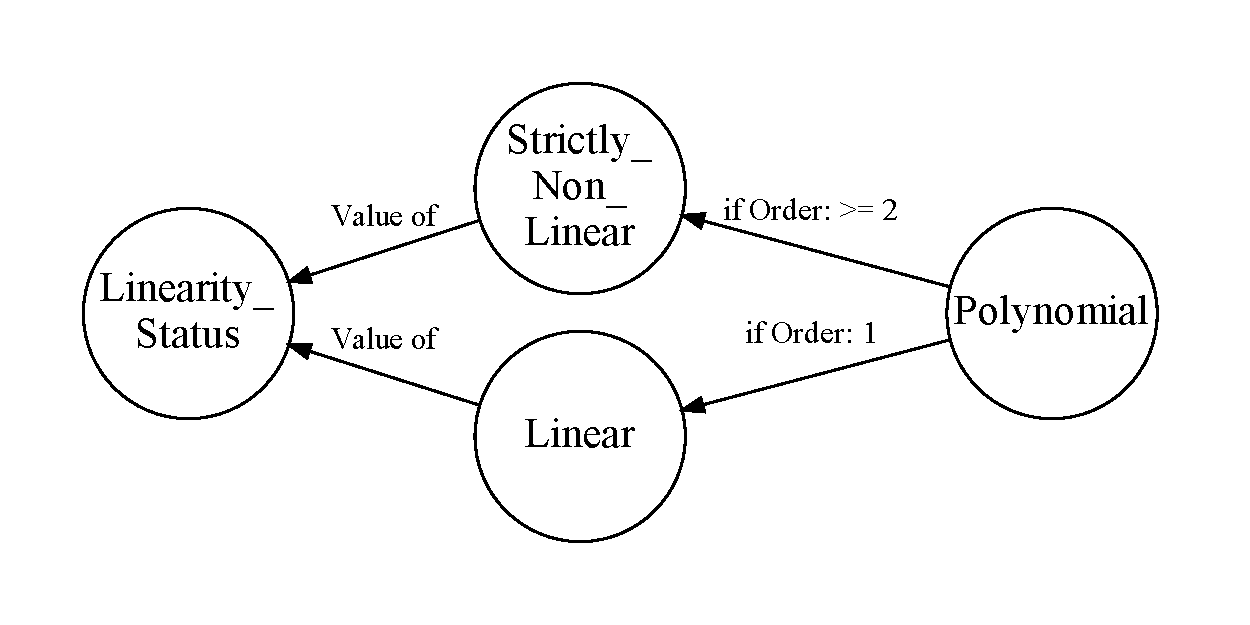
\includegraphics[width=1\linewidth]{Ausschnitt_KS_Poly_Linearity}
	\caption[Kategorie \textit{Polynom} im KS - verworfene Integrationsart]{Verworfene Integrationsart für die Kategorie \textit{Polynom} im KS}
	\label{fig:KS_Poly_False}
\end{figure}
Problemstellung: \textbf{Polynom}\\
Ein Polynom kann abhängig von seiner Ordnung linear oder nichtlinear sein. Um diesen Sachverhalt vollständig im KS abzubilden müsste das Polynom im KS ein Objekt der Kategorien \textit{Linear} und \textit{Strictly\_Non\_Linear} sein, welche zwei Werte der Kategorie \textit{Linearity} sind, die sich gegenseitig ausschließen. In der Anwendung auf ein Modell lässt sich dieser Widerspruch im Allgemeinen problemlos aufheben, da bei einem spezifischen Modell, dessen Modellgleichungen eine polynomiale Form haben, die Ordnung der Polynome festgelegt ist. Die durch diese Problemstellung aufgetretene Frage ist also: Sollen Widersprüche im KS auftreten dürfen, wenn diese sich bei Anwendung auf konkrete Modelle aufheben?
\begin{enumerate}[resume*]
	\item \label{E.KS_Widersprüche}Innerhalb KS soll es keine Widersprüche geben.
\end{enumerate}
Der Grund für die Entscheidung ist, dass es in Anbetracht der Anwendbarkeit für sinnvoller erachtet wurde das KS widerspruchsfrei zu gestalten. In Folge dieser Entscheidung wurde das Polynom der Kategorie \textit{Strictly\_Non\_Linear} zugeordnet.












